\documentclass[12pt, xcolor={dvipsnames}]{beamer}
\mode<presentation>{
  \usetheme{Madrid}
  % or ...
  \usecolortheme[named=OliveGreen]{structure}
  \setbeamercovered{transparent}
  % or whatever (possibly just delete it)
}
\usepackage[T2A,T1]{fontenc}
\usepackage[utf8x]{inputenc}

\usepackage[russian]{babel}

\usepackage{graphics}

\usepackage{wrapfig}
\usepackage{tikz}

\setlength{\parskip}{\baselineskip} 
%\usepackage[T1]{fontenc}
% or whatever

%\usepackage[latin1]{inputenc}
% or whatever

%\usepackage{times}
%\usepackage[T1]{fontenc}
% Or whatever. Note that the encoding and the font should match. If T1
% does not look nice, try deleting the line with the fontenc.


\title[] % (optional, use only with long paper titles)
{Анализ поверхности взаимодействия белков и поиск наиболее значительных позиций методом in silico Ala-scan}

%subtitle
%{Include Only If Paper Has a Subtitle}

\author[] % (optional, use only with lots of authors)
{
  \texorpdfstring{
	\begin{columns}
	\column{.55\linewidth}
		Магистрант:\\
		Научный руководитель:
	\column{.45\linewidth}
		Татьяна Малыгина, СПбАУ\\
		Павел Яковлев, BIOCAD
	\end{columns}
%	\\[30pt]
%    \begin{columns}
%        \column{.55\linewidth}
%        Место прохождения практики:
%        \column{.45\linewidth}
%        BIOCAD
%    \end{columns}
   }
   {\& }
}

% - Give the names in the same order as the appear in the paper.
% - Use the \inst{?} command only if the authors have different
%   affiliation.

%\institute[Universities of Somewhere and %Elsewhere] % (optional, but mostly needed)
%{
%  \inst{1}%
%  кафедра МиИТ, СПбАУ
%}
% - Use the \inst command only if there are several affiliations.
% - Keep it simple, no one is interested in your street address.

\date[DIPLOMA 2015] % (optional, should be abbreviation of conference name)
{СПбАУ, 2015}
% - Either use conference name or its abbreviation.
% - Not really informative to the audience, more for people (including
%   yourself) who are reading the slides online



% If you wish to uncover everything in a step-wise fashion, uncomment
% the following command: 

%\beamerdefaultoverlayspecification{<+->}
\setbeamertemplate{footline}[frame number]

\begin{document}
\begin{frame}
  \titlepage
\end{frame}
%\begin{frame}{Outline}
%  \tableofcontents
  % You might wish to add the option [pausesections]
%\end{frame}
\section{Введение}
\begin{frame}{Белки}{Некоторые важные определения}
\textbf{Первичная структура} белка задается последовательностью (\textbf{цепочкой}) аминокислот:

\resizebox{\textwidth}{!}{
%\input{aa3_5.tex}
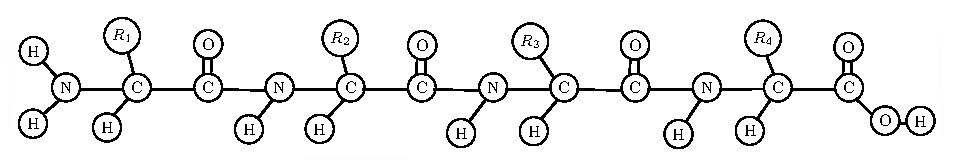
\includegraphics{aa3_1.eps}
}

\textbf{Вторичная структура} задается укладкой цепочки аминокислот в пространственные структуры, \textbf{третичная структура} - расположением этих структур в пространстве в случае, когда белок содержит только одну цепь.

Когда белок состоит из нескольких цепей, говорят о его \textbf{четвертичной структуре}.
\end{frame}

\begin{frame}{Белки и энергия}
С точки зрения химии, разным видам структуры соответствуют разные виды химических связей и электростатических взаимодействий.

Когда мы рассматриваем несколько цепочек в составе одного белка или несколько белков, образующих комплекс, мы говорим о \textbf{белок-белковом взаимодействии}.

\textbf{Интерфейс} такого взаимодействия -- это участки \textbf{поверхности} белков, непосредственно контактирующие между собой.

\end{frame}
\begin{frame}{Белок-белковое взаимодействие - I}
\begin{center}
\resizebox{!}{0.5\textheight}{
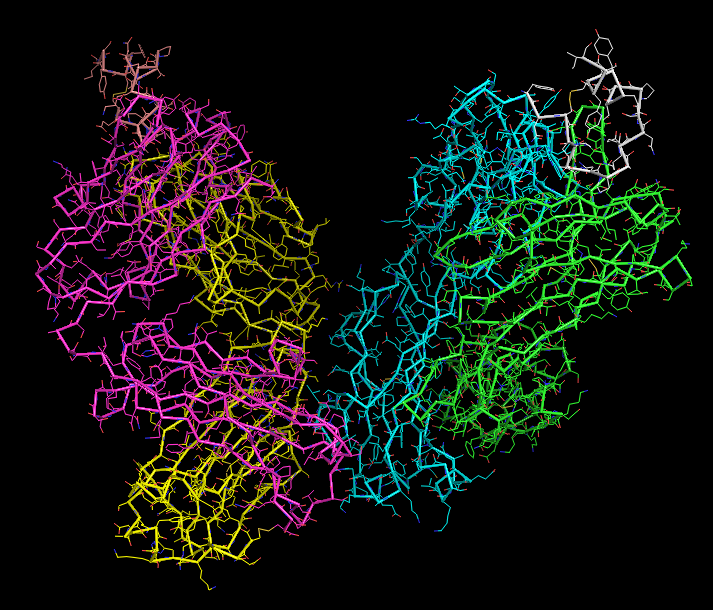
\includegraphics{antibody.png}
}
\end{center}
Рассмотрим белок, имеющий четвертичную структуру.

\textbf{Вопрос}: можно ли изменить что-то в его структуре, чтобы образующие его цепочки были лучше сцеплены между собой?
\end{frame}
\begin{frame}{Белок-белковое взаимодействие - II}
Пусть есть комплекс из двух белков (например, имунноглобулин и эпитоп).

\textbf{Вопрос 1}: можно ли изменить что-то в его структуре, чтобы усилить связь между компонентами комплекса?

\textbf{Вопрос 2}: насколько специфична одна из компонент комплекса?  Можно ли подобрать один из белков так, чтобы комплекс был более устойчивым? Насколько заменяема каждая из компонент?

Ответить нам поможет \textbf{аланиновое сканирование} (аланиновый мутагенез).
\end{frame}

\begin{frame}{Аланиновое сканирование}

Аланиновое сканирование (ала-скан)\footnote{2001, "Combinatorial alanine-scanning" (Morrison K.L., Weiss G.A.).}  - метод для определения аминокислот в составе белка, играющих важную роль в сохранении его функций, стабильности или формы.
\begin{wrapfigure}{RT}{0.3\textwidth}
\resizebox{0.3\textwidth}{!}{
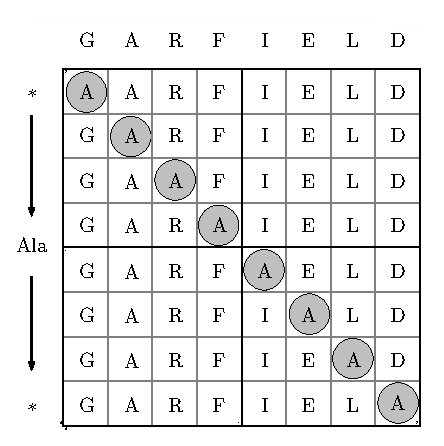
\includegraphics{ala_scan.eps}
}
\end{wrapfigure}

Проблемы ala-scan in vitro/in vivo:
\begin{itemize}
\item Большое пространство поиска.
\item Сложность синтеза библиотек: необходим индивидуальный подход!
\item Высокая стоимость.
\end{itemize}
\end{frame}
\begin{frame}{Энергетически горячие аминокислотные остатки}
Энергетически горячий остаток (ЭГО)\footnote{в англоязычной литературе ,,energy hotspot residue''} -- такая аминокислота в составе одного из компонент белок-белкового комплекса, мутагенез  которой приводит существенному изменению свободной энергии комплекса $\Delta\Delta G$.

Существенным обычно считают изменение, превышающее по модулю 0.5-1 килокалорий на моль.

Цель аланинового сканирования -- найти ЭГО.

Но для больших белков по всем аминокислотам его проводить долго, поэтому производится предварительный отбор аминокислот.
\end{frame}

\begin{frame}{Ala-scan in silico}{Компьютерное моделирование аланинового сканирования. Постановка задачи}
\textbf{На входе}: Пространственная структура белкового комплекса (в формате PDB).

\textbf{На выходе}: ЭГО.

\textbf{Как решить}: 
вычислить потери свободной энергии $\Delta\Delta G$ при замене аминокислотного остатка на аланин для всех аминокислот, выбрать позиции с существенным значением потери (как правило, существенным считают изменение больше 1 килокалории на моль).
\end{frame}

\begin{frame}{Ala-scan in silico}{Компьютерное моделирование аланинового сканирования. Методы}
"Computational alanine scanning of protein-protein interfaces" (Kortemme, et al. - 2004)

"Computational Alanine Scanning Mutagenesis - An Improved Methodological Approach" (I.S. Moreira, et al. - 2006)

Готовые решения используют (на этапе мутагенеза): 
\begin{itemize}
\item решения уравнения Пуассона-Больцмана (MM-PBSA)
\item метод возмущения свободной энергии
\item обобщенный метод Борна
\item метод Монте-Карло
\end{itemize}
Посмотрим, как выбирают области для аланинового сканирования.
\end{frame}
\begin{frame}{Выбор регионов для сканирования I}{Использование отсечки по расстоянию}
\begin{itemize}
\item Аланиновому сканированию подвергаются аминокислоты цепочки, образующей комплекс совместно с другой цепочкой, содержащие атомы, удаленные от каких-либо атомов цепочки, также участвующей в образовании комплекса, на расстояние, не превышающей некоторой фиксированной величины

\item В качестве порогового значения расстояния используются, например, величины 4, 5, 8 A

\item в Rosetta Alascan Protocol используется усложнение: дополнительно рассматриваются аминокислоты, $\beta$-углерод которых после формирования комплекса в шаре определенного фиксированного радиуса содержит существенно больше атомов $\beta$-углерода, чем содержал до этого.
\end{itemize}
%Почему проводят не по всем позициям
%как выбирают
%методы
\end{frame}
\begin{frame}{Эксперимент}
\begin{itemize}
\item Рассмотрим базу данных с информацией о результатах эспериментов по аланиновому сканированию ASEdb.
\item Найдем объекты со ссылкой на Protein Data Bank.
\item Среди всех таких объектов, найдем те, в которых есть аминокислоты, мутация которых приводит к существенному изменению свободной энергии комплекса ($\geq 1$ ккал/моль)
\item Посмотрим, всегда ли они удалены от интерфейса в пределах стандартно используемой отсечки (в качестве примера возьмем расстояние, не превышающее 8 \AA{}).
\end{itemize}
\end{frame}
\begin{frame}{Результаты эксперимента}
Комплекс человеческого гормона роста и рецептора человеческого гормона роста\footnote{идентификатор структуры в Protein Data Bank -- 3hhr}
%1. картинка с примером
\begin{center}
\resizebox{!}{0.5\textheight}{
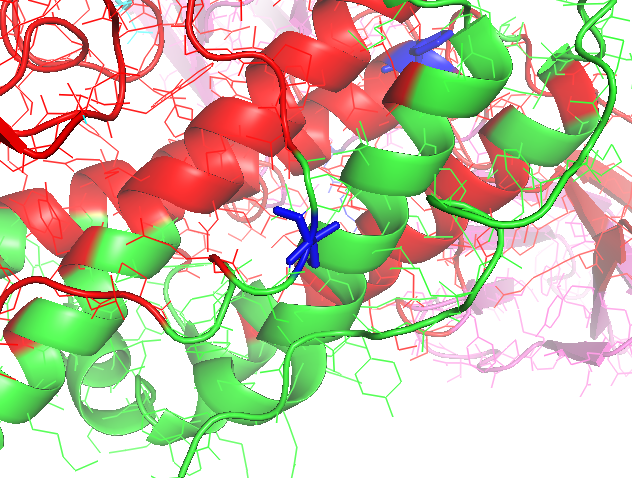
\includegraphics{image7.png}
}
\end{center}
\end{frame}

\begin{frame}{Выбор регионов для сканирования II}{Поиск по гомологии}

ASEdb: 76/101 корректных записей о белках, из них много 3hhr.

Еще одна замечательная база данных:
\begin{center}
\resizebox{!}{0.6\textheight}{
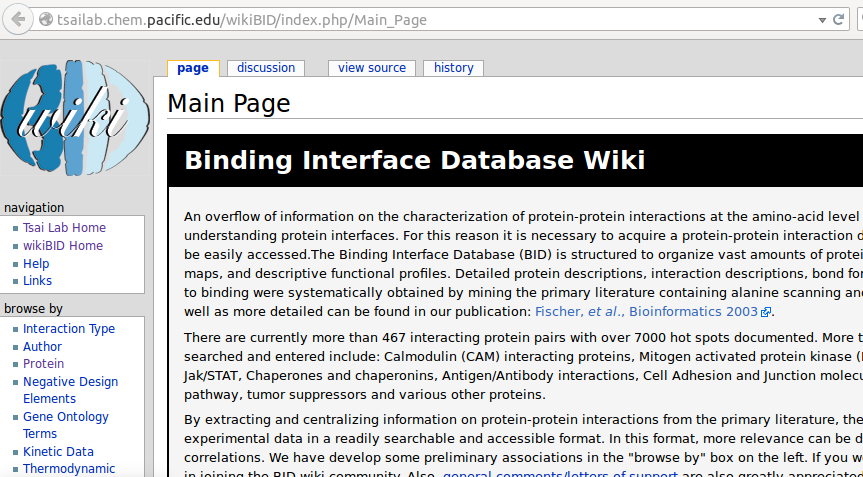
\includegraphics{exp2.png}
}
\end{center}
\end{frame}

\begin{frame}{Выбор регионов для сканирования II}{Выводы. Основная задача.}

Выводы: эффективного и универсального метода способа найти ЭГО -- не придумали.

Будем решать эту задачу. Для этого попробуем по полученной картинке понять, что еще необходимо учесть:
%1. картинка с примером
\begin{center}
\resizebox{!}{0.5\textheight}{
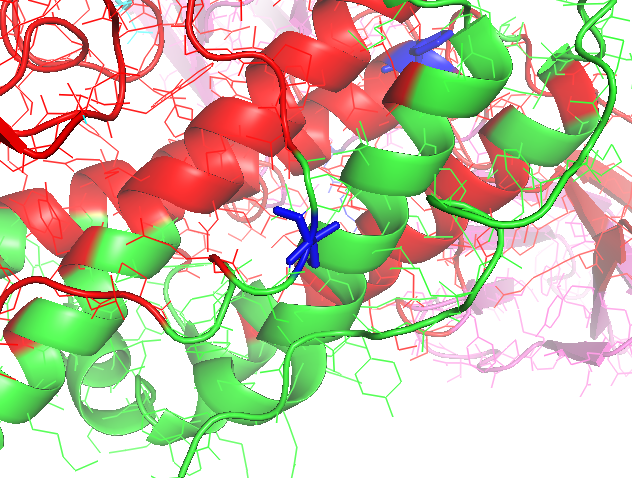
\includegraphics{image7.png}
}
\end{center}
\end{frame}

\begin{frame}{Как будем выбирать регионы для сканирования}
\begin{itemize}
\item разумно начинать с области интерфейса белок-белкового взаимодействия, затем расширять ее.
\item при мутации не гидрофобные аминокислоты могут стать гидрофобными и оказаться значимыми, поэтому в первую очередь можно расширить область на такие аминокислоты, находящиеся на границе интерфейса.
\item поскольку при выборе интерфейса с отсечкой по расстоянию в интерфейсе могут появляться дыры, будем их заполнять. Для этого будем искать поверхностные карманы (углубления в поверхности белка в границах интерфейса).
\item Из всех вторичных структур на поведение белка больше всего влияют петли. Добавим в интерфейс все аминокислоты, содержащиеся в петлях, которые частично уже попали в область рассмотрения.
\end{itemize}
\end{frame}


\begin{frame}{Алгоритм поиска протяженных регионов,}{ потенциально содержащих ,,энергетически горячие точки''}
Включим в состав множества протяженных регионов, содержащих ,,энергетически горячие аминокислотные остатки'', следующее:
\begin{itemize}
\item аминокислоты, образующие ,,интерфейс'' взаимодействия с парной цепочкой или белком (с использованием отсечки по расстоянию от второй цепочки)
\item аминокислоты, образующие поверхность ,,карманов'', находящихся в области взаимодействия пары белков
\item не-гидрофобные аминокислоты, являющиеся соседними по отношению к аминокислотам, образующим интерфейс
\item если интерфейс взаимодействия образован петлями, то добавим все аминокислоты, образующие петли 
\end{itemize}


\end{frame}
\begin{frame}{,,Интерфейс''}
\begin{itemize}
\item определяем множество треугольников выпуклой оболочки, для которых хотя бы одна вершина удалена от центров атомов второй цепочки не больше, чем на выбранное значение отсечки
\item Далее расширяем интерфейс
\begin{itemize}
\item шаг 1: добавляем к интерфейсу все треугольники выпуклой оболочки, содержащие атомы аминокислот, которые уже туда попали
\item шаг 2: продлеваем регион до границы гидрофобности
\item шаг 3: продлеваем регион за границы гидрофобности на 1 аминокислоту.
\end{itemize}
\end{itemize}


В результате у нас есть одна или нескольких протяженных связных областей выпуклой оболочки, по которым можно восстановить аминокислоты.
\end{frame}


\section{Поиск регионов}
\begin{frame}{Триангуляция Делоне}
\begin{itemize}
\item Рассматриваем одновременно 2 цепочки, образующие белковый комплекс.
\item Начнем с построения выпуклой оболочки и триангуляции Делоне для каждой из них, будем искать протяженные регионы с энергетически горячими аминокислотными остатками  на одной из них. Строить будем по центрам атомов, формирующих аминокислоты цепочки.
\item Выберем все треугольники выпуклой оболочки, в которых хотя бы одна вершина удалена от некоторых атомов второй цепочки не далее, чем на выбранное (фиксированное) значение отсечки.
\end{itemize}
\end{frame}

\begin{frame}{Построение графа по триангуляции Делоне}
\begin{center}
\resizebox{!}{0.5\textheight}{
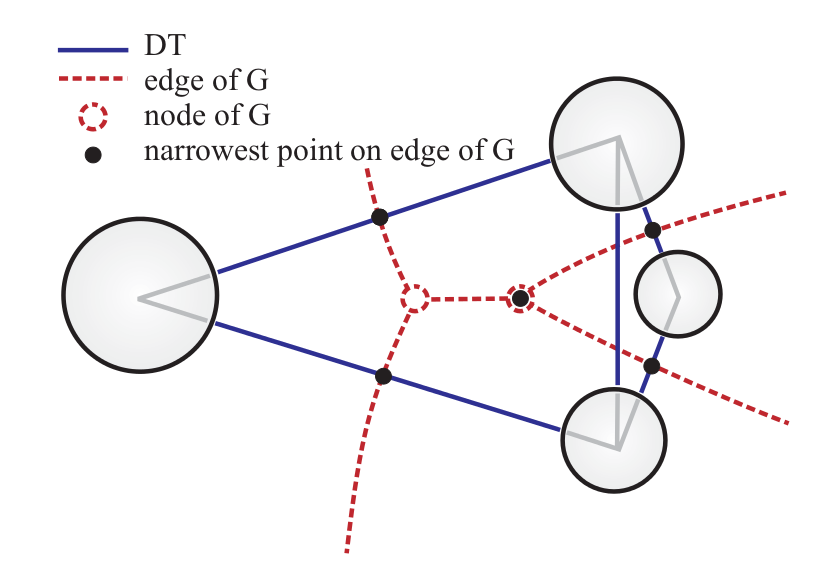
\includegraphics{image4_caver.png}
}

[Computation of tunnels in protein molecules using
Delaunay triangulation, P.Medek, et al., 2007]
\end{center}

Используем модифицированный алгоритм Дейкстры, аналогично упомянутому в оригинальной работе.
\end{frame}

\begin{frame}{Петли}

Перед добавлением петель треугольники триангуляции преобразуются в фрагменты последовательности аминокислот, продлеваем их, используя информацию о вторичной структуре.

\end{frame}
\section{Аланиновое сканирование}

\begin{frame}{Ala-scan in silico с фильтрацией данных}{Реализация}
\textbf{Полученный алгоритм аланинового сканирования} основан на Rosetta alascan protocol и образован следующей последовательностью действий:
\begin{itemize}
\item читаем 2 цепочки атомов из PDB,
\item выбираем аминокислоты одной из цепочек с помощью приведенного выше алгоритма поиска,
\item для этих аминокислот пробуем провести мутагенез с использованием метода Монте-Карло выводим те, изменение которых привело к существенным изменениям свободной энергии системы.
\end{itemize}
\end{frame}

\begin{frame}{Результаты}
\begin{itemize}
\item Получен скрипт, который итеративно формирует протяженные регионы, содержащие ЭГО (в процессе тестирования), и который может использоваться в модифицированном rosetta ala-scan protocol для поиска аминокислотных последовательностей.
\item Планируется: переделать в плагин к PyMol, добавить промежуточный вывод аминокислот для визуального воспроизведения (в виде mesh-объекта)
\item Предоположительно, в алгоритм можно добавить поиск по гомологии (на стадии идеи)
\end{itemize}
\end{frame}

\section{Результаты}
%здесь должны быть скриншоты из PyMol,
%на которых видно выделение областей в отдельный mesh

\begin{frame}{}
Вопросы?
\end{frame}

\end{document}

